\chapter{Methoden}
\label{cha:Methoden}

In diesem Kapitel werden die Grundlagen vermittelt, welche für das Verständnis der Arbeit in ihrer Gänze notwendig sind.
%und Evaluation der Arbeit von Bedeutung sind.

\section{Aminosäurerest-Pseudopotentiale}

Bei den \acf{APs} handelt es sich um eine Methode der Transformation der physikochemischen und wechselwirkenden Eigenschaften, von den Aminosäuren in der Proteinstruktur, in ein Energiemaß. Diese Energiemaße werden dabei durch eine dimensionslose Dezimalzahl dargestellt und im Gegensatz zur hochkomplexen 3D-Strukturen sind die Berechnungen mit ihnen unmittelbarer. Die Energieprofile stehen auf dem Webserver \emph{eProS}\footnote{\url{https://biosciences.hs-mittweida.de/epros/}} zum Download bereit. Zusätzlich wurde zur lokalen Berechnung und zu Testzwecken eine Möglichkeit von den Entwicklern der \ac{bigM}\footnote{\url{http://www.bioforscher.de/bigM/}}, zur Berechnung der Energieprofile, zur Verfügung gestellt.

Durch die \ac{APs} können zu den lokalen Interaktionen der direkten Nachbarn, auch noch die globalen Interaktionen der indirekten Nachbarn hinzugezogen werden. Zur Berechnung benutzt man die Betrachtung einer 8 Angström Sphäre, siehe Abb. \ref{fig:8A_Sphaere}, um die betreffende Aminosäure herum und analysiert ob noch andere Aminosäuren des Proteins in diese Sphäre hineinragen. Somit können auch Effekte wie sterische Hinderung berücksichtigt werden. Durch diese neue Sichtweise löst man sich von der starren Betrachtungsweise der Sequenz und der 2D-Struktur, wie es bei bisherigen Vorhersage-Algorithmen war.

\begin{figure}
    \centering
    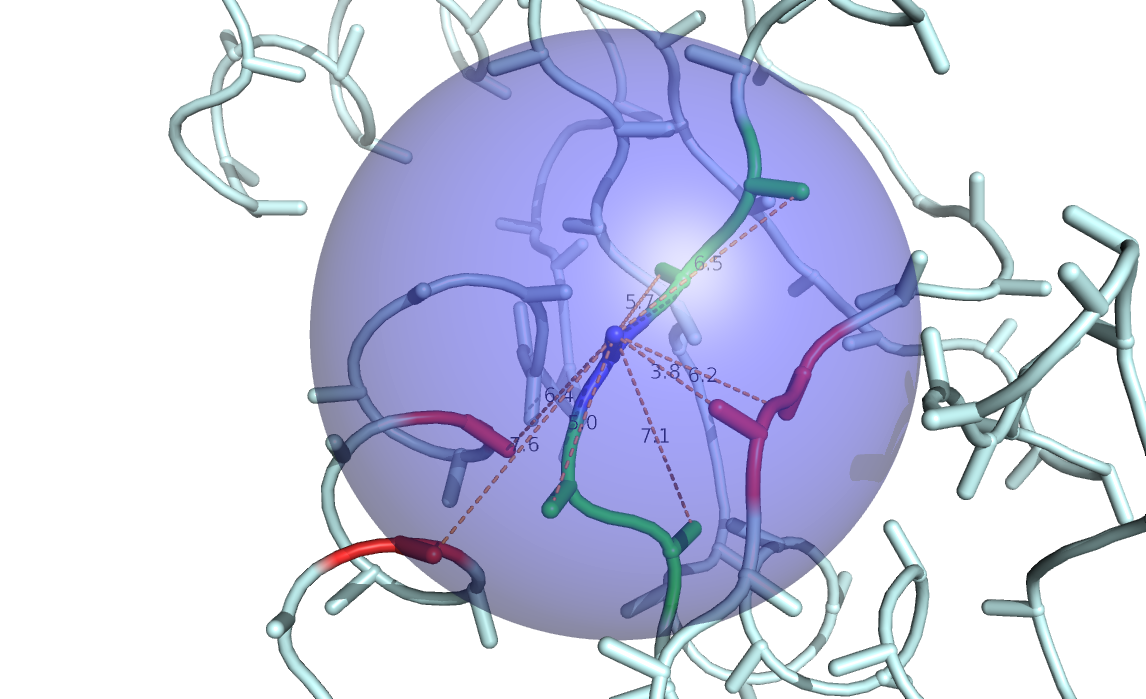
\includegraphics[width=.95\textwidth]{8A_Sphaere.png}
    \caption{Ein 3D Modell einer Proteinstruktur, hellblau ist die 8 Angström Umgebung um die dunkelblaue Aminosäure im Zentrum, mit direkten Nachbarn in grün und in indirekten Nachbarn in rot. Die punktierte Linie zeigt den Abstand der $C_{\alpha}$ Atome in Angström.}% \cite{8A_Sphaere}
    \label{fig:8A_Sphaere}
\end{figure}

Energieprofile sind grobkörnige Aminosäure-Interaktionsmodelle, basierend auf $C_{\alpha}$ und $C_{\beta}$ Atom Koordinaten, welche aus bekannten Proteinstrukturen extrahiert werden. Es wird die natürlich Neigung eines Aminosäurerests, mit anderen Resten zu interagieren, untersucht. Bei Membran lokalisierten Proteinen wird zusätzlich noch, die Neigung der Aminosäureresten sich in Richtung der Lipiddoppelschicht zu richten, berücksichtigt. 

Generell ist die Energie abhängig von der Neigung des Aminosäurerests nach außen ($n_{out}$), in das umgebende Milieu oder in das Innere ($n_{in}$) des Proteins. Nimmt man nun den negativen natürlichen Logarithmus zur Basis 10, so ergibt sich für $e_{a_i}$ folgende Gleichung \ref{eq:definition}:
%
\begin{equation}
  	e_{a_i} \propto -\ln{\left(\frac{n_{a_i}^{in}}{n_{a_i}^{out}}\right)}
  	\label{eq:definition}
\end{equation}

Diese Parameter sind von bekannten globularen- und membranassoziierten Proteinen hergeleitet. Wie in \ref{eq:single} zu sehen, ist die Interaktionsenergie $e_{a_{i}}$, $a_{j}$ zwischen 2 Aminosäuren $a_{i}$ und $a_{j}$ gleich der Summe ihrer beiden Energien. 

\begin{equation}
  	e_{a_{i},a_{j}} = \left( e_{a_{i}} + e_{a_{j}} \right)
    \label{eq:single}
\end{equation}

Somit lässt sich die Gesamtenergie des Aminosäurerests $E_{a_i}$ mittels \ref{eq:total} berechnen:

\begin{equation}
    E_{a_{i}} = \sum_{< i, j >}{e_{a_{i},a_{j}}}
    \label{eq:total}
\end{equation}

In ihren Arbeiten hat das ePros Team Mittweida gezeigt, dass die \ac{APs} genutzt werden können, um die Proteinstruktur Stabilität und Funktionalität zu untersuchen. Es wurde gezeigt, dass Ähnlichkeiten der Energieprofile von Proteinen auf Ähnlichkeiten der strukturellen und funktionellen Eigenschaften dieser Proteine deuten \cite{Heinke.2011}.


\subsection{ePros Webserver}
\label{sec:epros}
Die einzige aktuelle Quelle fertig berechneter Energieprofile ist der ePros Webserver\footnote{\url{https://biosciences.hs-mittweida.de/epros}}. Mittels ePros lassen sich nicht nur Energieprofile für bestimmte \ac{PDB} IDs abrufen, sondern auch noch einige andere Tools nutzen.

\begin{figure}
    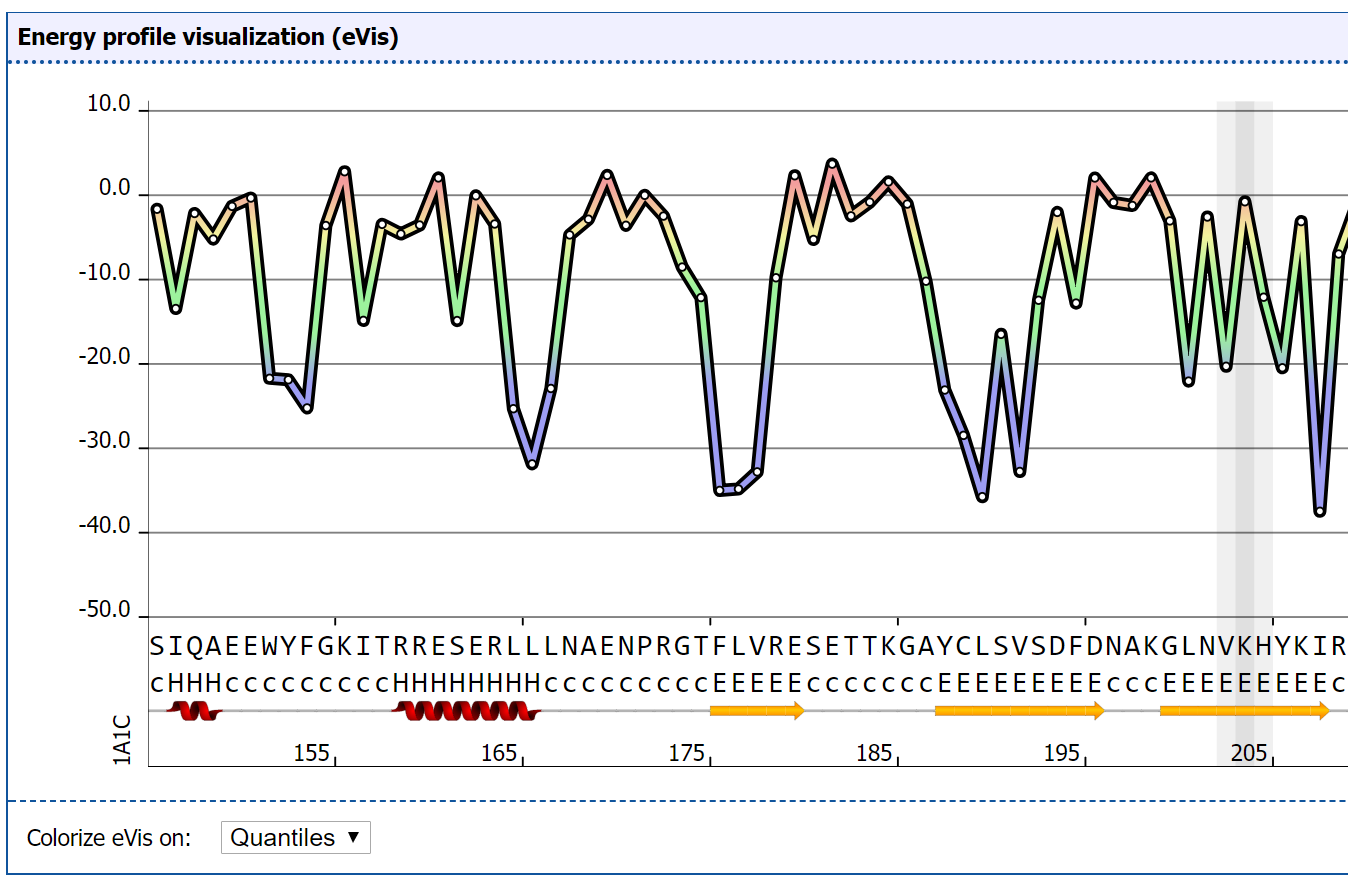
\includegraphics[width=.95\textwidth]{images/ePros.png}
    \caption{Dargestellt ist ein Ausschnitt aus dem Protein \texttt{1A1C}, welches mit \ac{eVis} visualisiert wurde. Auf der Abszisse sind die Aminosäuren im Einbuchstabencode aufgetragen, siehe Tabelle \ref{tab:amino_table}. Darunter ist die Sekundärstruktur als Buchstabencode und als Visualisierung aufgetragen. Unten ist die Aminosäureposition in 10er Schritten aufgetragen. Auf der Ordinate befinden sich die berechneten Energiewerte.}
    \label{fig:epros}
\end{figure}

\begin{description}
    \item[eCalc]
    Mittels \emph{eCalc} lassen sich Energieprofile auf Grundlage einer Struktur oder \ac{PDB} ID berechnen. Das EP wird dann in einem 2D-Graphen visualisiert, sodass man leicht die Energiewerte jeder Aminosäure sehen kann, sowie deren Sekundärstruktur, siehe Abb. \ref{fig:epros}.
    \item[eAlign]
    Mit \emph{eAlign} ist es möglich, zwei EPs mit einem modifizierten Needle-man-Wunsch/Smith-Waterman Algorithmus zu alignieren und paarweise zu vergleichen.
    \item[eGOR]
    Anders als \emph{eCalc}, ist \emph{eGOR} ein \emph{GOR} \cite{Garnier.1996} basierter Ansatz, um ein EP zu berechnen, als Grundlage dient eine Aminosäuresequenz.
    \item[eSearch]
    Dieses Tool führt paarweise Vergleiche eines gegebenen EPs mit der vorberechneten eProS-Datenbank durch. Nach der Berechnung werden die besten Treffer visualisiert und können detaillierter analysiert werden.
    \item[eMut]
    Mit \emph{eMut} lassen sich die energetischen Ähnlichkeiten und Unterschiede von Proteinen gleicher Länge anzeigen. Erkannte energetische Veränderungen könnten einen Einblick in funktionale und strukturelle Divergenzen geben.
\end{description}


\subsection{Energieprofile}
\label{sec:Energieprofil}
Energieprofile (EPs) sind die Grundlage dieser Arbeit, daher wird kurz der Aufbau des Datenformats erklärt. Ein \ac{EP} ist eine Datei mit \ac{APs} für jede Aminosäure. Im folgenden Beispiel ist das \ac{EP} für die Struktur \texttt{3T4F} der \emph{F Chain} dargestellt. Die ersten beiden Zeilen beschreiben das \ac{EP}, in der ersten Zeile steht der Name der Struktur und in der Zweiten ob es sich um ein globuläres oder alpha helikales Protein handelt. Die restlichen Zeilen sind immer gleich aufgebaut und Tabstopp separiert. In der Spalte steht immer \texttt{ENGY}, gefolgt von dem Chain Buchstaben, dahinter steht die Aminosäurennummer und der Aminosäurennamen. Dahinter steht die Sekundärstruktur und ganz am Ende steht der Energie Wert der betreffenden Aminosäure. Am Ende der Datei können noch Zeilen mit \texttt{REMK} beginnen, in denen z.B. die Qualität der zugrundeliegenden \ac{PDB} Datei angegeben ist.

\begin{table}[]
    \centering
    \caption{Gezeigt ist ein \acf{EP} des globulären Proteins \texttt{3t4f}, zu sehen in den obersten beiden Zeilen. Die dritte Zeile enthält die Header Zeile, welche Aufschluss über die folgenden Zeilen gibt, welche immer gleich aufgebaut sind. Die \texttt{ENGY} Zeilen beginnen mit dem Aminosäureketten-Buchstaben, gefolgt von der Position, dem Namen, der Sekundärstruktur und dem Energiewert der Aminosäure.}
    \label{tab:EP}
    \begin{tabular}{llllll}
    NAME & 3t4f &  &  &  &  \\
    TYPE & globular &  &  &  &  \\
    HEAD & Chain & ResNo & Res & SS & Energy \\
    ENGY & F & 1 & P & c & -0.36651769255470024 \\
    ENGY & F & 3 & G & c & -1.7143933253759942 \\
    ENGY & F & 4 & P & c & -0.4886902567396003 \\
    ENGY & F & 6 & G & c & -1.7143933253759942 \\
    ENGY & F & 7 & P & c & -0.426609617950302 \\
    ENGY & F & 9 & G & c & -0.8189007383286611 \\
    ENGY & F & 10 & P & c & 0.8896661049247689 \\
    ENGY & F & 11 & K & c & 5.678058211612121 \\
    ENGY & F & 12 & G & c & 0.3188212258358888 \\
    ENGY & F & 13 & E & c & 2.612350424331274 \\
    ENGY & F & 15 & G & c & -1.3849755172085403 \\
    ENGY & F & 16 & P & c & -0.4886902567396003 \\
    ENGY & F & 18 & G & c & -1.7143933253759942 \\
    ENGY & F & 19 & P & c & -0.6108628209245004 \\
    ENGY & F & 21 & G & c & -1.7143933253759942 \\
    ENGY & F & 22 & P & c & -0.4886902567396003 \\
    ENGY & F & 24 & G & c & -0.735024098503097
    \end{tabular}
\end{table}

\begin{table}[]
    \centering
    \caption{Die 20 kanonischen Aminosäuren mit Abkürzungen, Acylgruppe und prozentualer Anteil an der Gesamtheit\protect\footnotemark. Diese Tabelle dient dem Verständis der Tabelle \ref{tab:EP}, \ac{Abb} \ref{fig:epros}, \ac{Abb} \ref{fig:energy_ranges} und \ac{Abb} \ref{fig:ep_vs_snp}.}
    \label{tab:amino_table}
    \resizebox{\linewidth}{!}{%
    \begin{tabular}{llllll}
     &  &  &  &  &  \\
     &  &  &  &  &  \\ \hline
    \multicolumn{1}{|l|}{Name} & \multicolumn{1}{l|}{Abk.} & \multicolumn{1}{l|}{Symbol} & \multicolumn{1}{l|}{Acylgruppe} & \multicolumn{1}{l|}{essentiell?} & \multicolumn{1}{l|}{Ø in Proteinen} \\ \hline
    Alanin & Ala & A & Alanyl- & nein & 9,0 \% \\
    Arginin & Arg & R & Arginyl- & semi & 4,7 \% \\
    Asparagin & Asn & N & Asparaginyl- & nein & 4,4 \% \\
    Asparaginsäure & Asp & D & $\alpha$-Aspartyl- & nein & 5,5 \% \\
    Cystein & Cys & C & Cysteinyl- & nein & 2,8 \% \\
    Glutamin & Gln & Q & Glutaminyl- & nein & 3,9 \% \\
    Glutaminsäure & Glu & E & $\alpha$-Glutamyl- & nein & 6,2 \% \\
    Glycin & Gly & G & Glycyl- & nein & 7,5 \% \\
    Histidin & His & H & Histidyl- & semi & 2,1 \% \\
    Isoleucin & Ile & I & Isoleucyl- & ja & 4,6 \% \\
    Leucin & Leu & L & Leucyl- & ja & 7,5 \% \\
    Lysin & Lys & K & Lysyl- & ja & 7,0 \% \\
    Methionin & Met & M & Methionyl- & ja & 1,7 \% \\
    Phenylalanin & Phe & F & Phenylalanyl- & ja & 3,5 \% \\
    Prolin & Pro & P & Prolyl- & nein & 4,6 \% \\
    Serin & Ser & S & Seryl- & nein & 7,1 \% \\
    Threonin & Thr & T & Threonyl- & ja & 6,0 \% \\
    Tryptophan & Trp & W & Tryptophyl- & ja & 1,1 \% \\
    Tyrosin & Tyr & Y & Tyrosyl- & nein & 3,5 \% \\
    Valin & Val & V & Valyl- & ja & 6,9 \%
    \end{tabular}}
\end{table}
%\footnotetext{\url{https://de.wikipedia.org/wiki/Aminosäuren##Kanonische_Aminos.C3.A4uren}}




\newpage
\section{Datenbanken}
Bei dem Aufbau eines passenden Datensatzes wurden die Datenbanken \ac{PDB} und \ac{Pfam} genutzt, welche zusammen als Datengrundlage für die spätere $\psi$ \& $\phi$ Winkel Kalkulation dienten. Zusätzlich war die ClinVar Datenbank noch essentiell, denn sie diente als Grundlage für die \ac{SNP} Daten.


\subsection{RCSB PDB}

Eine wichtige Grundlage der Arbeit ist die „Protein Daten Bank“, kurz PDB \cite{Bernstein.1977}. Sie enthält die 3D-Strukturdaten der Proteine, welche die Grundlage der Energieprofile sind. Die \ac{PDB} enthält zusätzlich noch Strukturdaten von Nukleinsäuren und \emph{complex Assemblies}\cite{Kim.2009}, die in allen Aspekten der Biomedizin und der Landwirtschaft, von der Proteinsynthese bis hin zum Gesundheitswesen, von Bedeutung sind. Die \ac{PDB} bietet auf Grundlage dieser Daten Tools für Forschung und Bildung in der Molekularbiologie, in der Strukturbiologie und in der Rechenbiologie an.
Die \ac{PDB} wurde 1971 von den \ac{BNL}\footnote{\url{https://www.rcsb.org/pdb/static.do?p=general_information/about_pdb/index.html}} als Archiv für biologische makromolekulare Kristallstrukturen etabliert und beinhaltete anfangs nur 7 Strukturen. 1980 zeigte sich ein rasanter Anstieg der eingereichten Strukturen, ausgelöst durch einen verbesserten Prozess der Kristallographie, einen offeneren Datenaustausch der wissenschaftlichen Gemeinschaft und der neuen Methode der Kernspinresonanzspektroskopie. So umfasst der Datensatz zum Zeitpunkt der vorangegangenen Arbeit 101.207 Strukturen (Juni 2014) und zum heutigen Zeitpunkt über 133.920 Strukturen (Oktober 2017). Bei einem Wachstum von fast 10.000 Strukturen pro Jahr, macht dies die \ac{PDB} zur weltweit größten Sammlung von bekannten Proteinstrukturen.

\begin{figure}
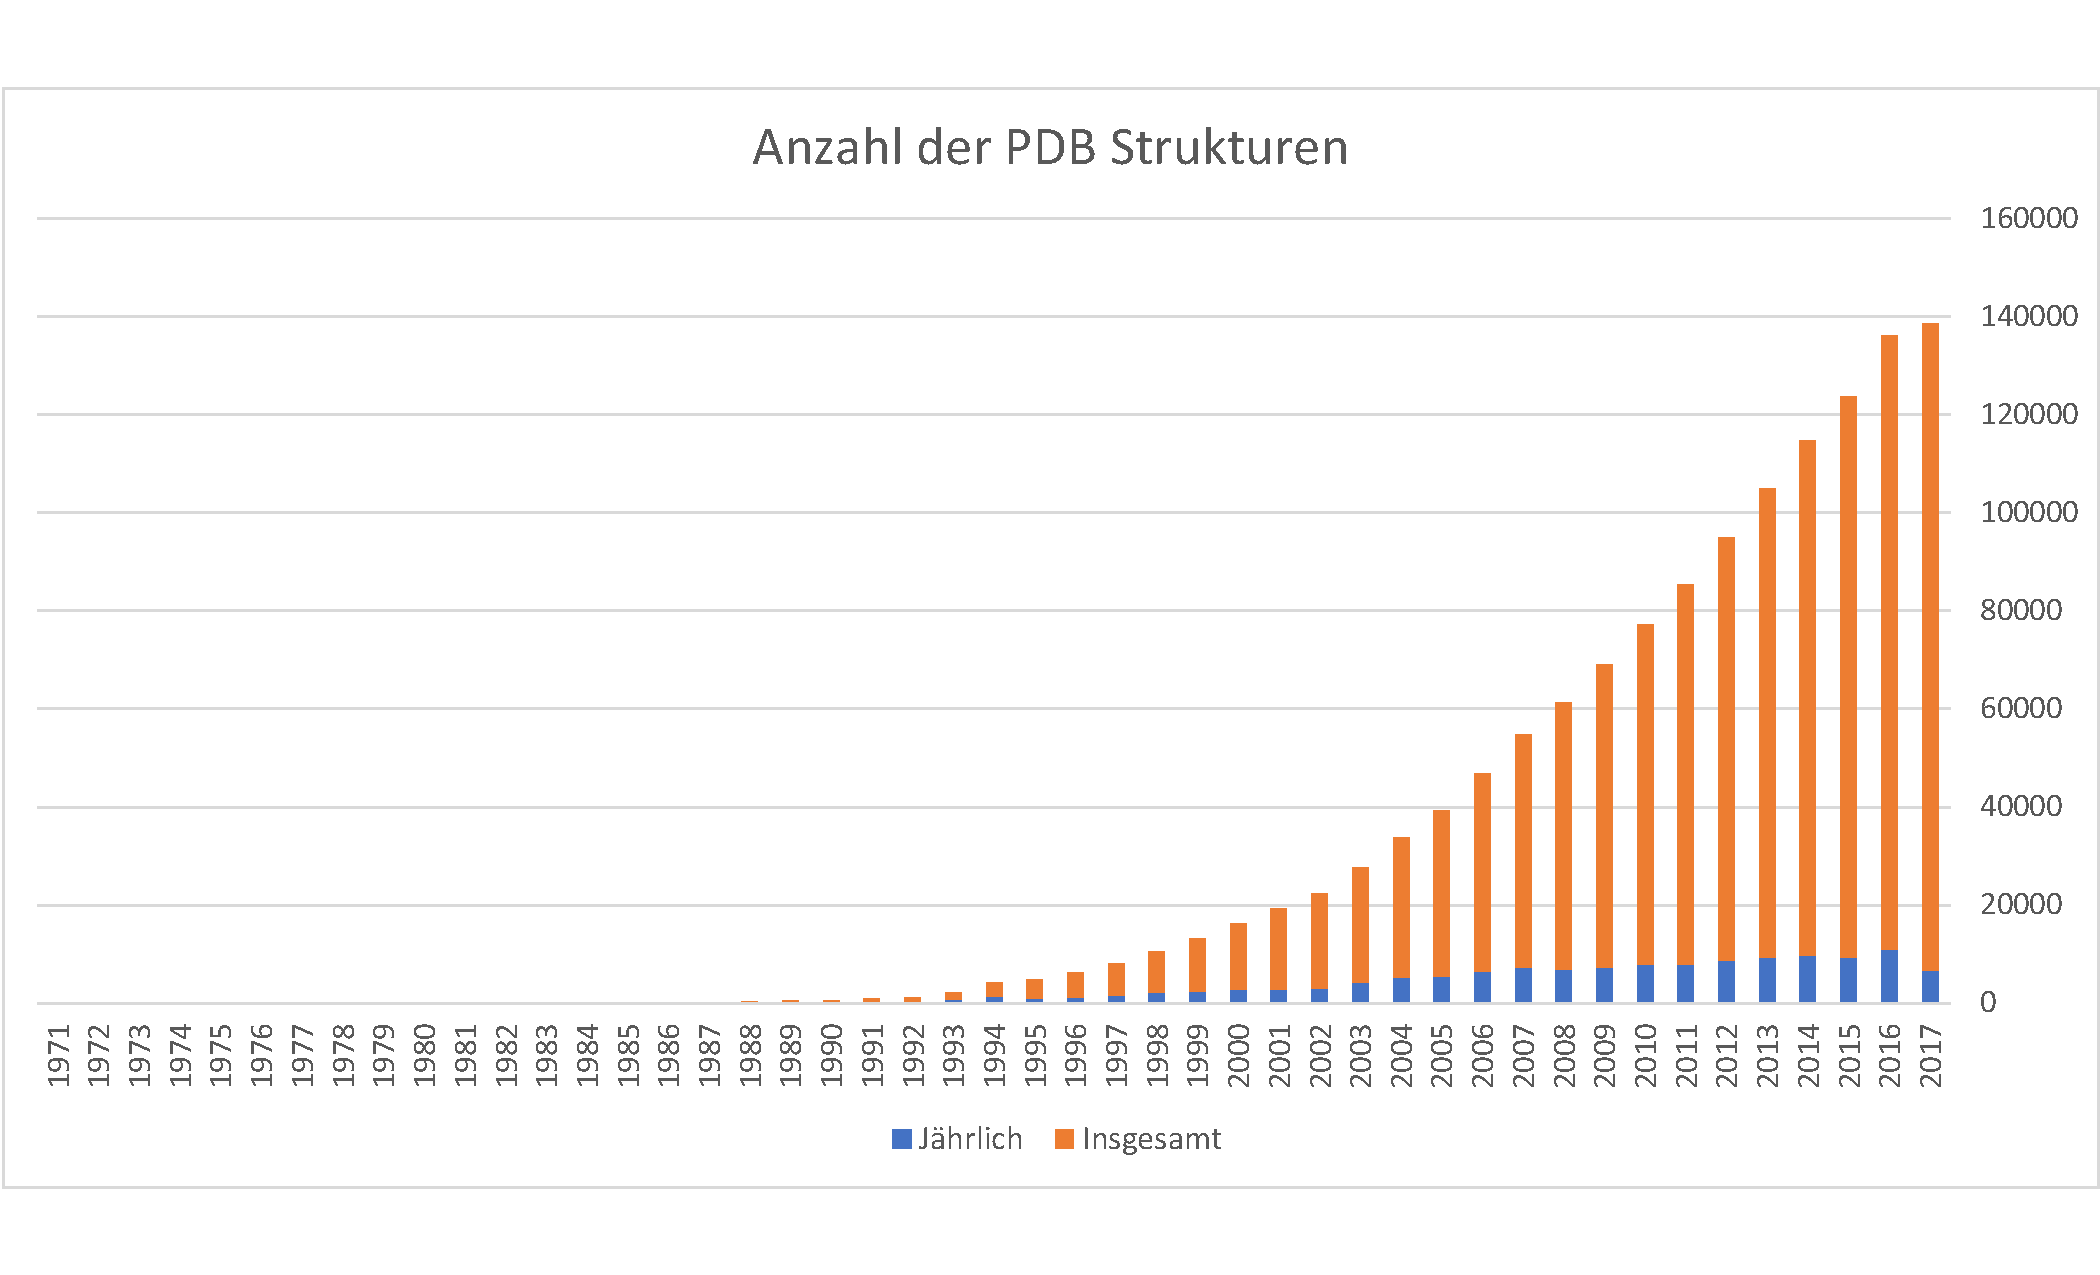
\includegraphics[width=.95\textwidth]{PDB_growth_rate.pdf}
%\caption{}
\caption{Die jährliche Wachstumsrate\protect\footnotemark \ der \ac{PDB} seit ihrer Gründung 1971 bis 2017. Auf der Abszisse sind die Jahre aufgetragen und auf der Ordinate sind die Strukturen pro Jahr (blau) und insgesamt (orange) abgebildet.}
\label{fig:PDB_growth_rate}
\end{figure}

%Der Zugriff auf die \ac{PDB} hat sich im Laufe der Jahre drastisch geändert, so wurden die Daten am Anfang noch mit Magnet Medien ausgetauscht, so kam mit der Etablierung des WWW, der Datenaustausch über dieses. Ebenso haben sich die Autoren der Daten geändert, so waren es am Anfang nur Experten auf dem Fachgebiet der Strukturellen Forschung, so sind es heute unterschiedlichste Kompetenzen in den Techniken der Röntgenkristallstrukturbestimmung, Kernspinresonanz, Kryo-Elektronenmikroskopie und theoretischen Modellierung. Genau so hat sich auch die Nutzerschaft erweitert, sodass es heute eine sehr diverse Gruppe aus Forschern, Lehrern und Studenten in den Fachbereichen Biologie, Chemie, Informatik und Physik ist. Die zunehmende Erkenntnis über den Wert der Daten und dem daraus resultierenden Verständnis der biologischen Funktion, sorgte für einen erhöhten Zustrom an Daten und erforderte einen neuen Weg die Daten zu sammeln, organisieren und zu verteilen. 
Im Oktober 1988 wurde das Management der \ac{PDB} zuständig für die \ac{RCSB}. Die \ac{PDB} setzt sich heute aus einer Vielzahl von Unterdatenbanken zusammen. Die wichtigsten sind die europäische \ac{PDB} (PDBe), die japanische \ac{PDB} (PDBj), die Biological Magnetic Resonance Bank (BMRB) und die worldwide \ac{PDB} (wwPDB). Zusammen pflegen und kuratieren diese Datenbanken die \ac{PDB} und sorgen dafür, dass die \ac{PDB} weltweit frei und öffentlich verfügbar ist.

%Die Vision der RCSB ist es eine Ressource zu schaffen, welche mittels modernster Technologien, die Nutzung und Analyse von Strukturdaten erleichtert und damit eine Grundlage für die biologische Forschung stellt. 
\footnotetext{Die Daten der Tabelle befinden sich auf der offiziellen Webseite der RCSB \ac{PDB} unter: \url{http://www.rcsb.org/pdb/statistics/contentGrowthChart.do?content=total}}

In dieser Arbeit wurde mit dem \ac{PDB} Dateiformat gearbeitet, dieses wird im folgenden Abschnitt kurz erklärt. Alle Strukturen der \ac{PDB} sind im \texttt{.pdb} Format verfügbar. Dieses ist sehr strikt geregelt, jede Zeile darf maximal 80 Zeichen enthalten und muss mit einem Identifyer beginnen. Anders als bei ähnlichen Formaten, werden hier einzelne Spalten nicht durch Tabs separiert, sondern befinden sich an genau charakterisierten Positionen. 
%Z.B. ist der \emph{Residue name} in der \texttt{ATOM} Zeile immer an der Position 18-20 zu finden, wobei die 1. Position bei 1 beginnt und nicht bei 0. 
Für weitere Arbeiten ist die Seite 176 in den Formatvorgaben\footnote{Die Formatvorgabe ist zu finden unter \url{ftp://ftp.wwpdb.org/pub/pdb/doc/format_descriptions/Format_v33_A4.pdf}} der \ac{PDB} interessant.


\subsection{Pfam}
\label{sec:pfam}
Die Protein Family Database \cite{Finn.2014} oder kurz Pfam enthält nah-verwandte Sequenz Alignments, sogenannte Proteinfamilien. Diese setzen sich aus einem repräsentativen Subset aus einem Satz übereinstimmender Sequenzen zusammen, dem sogenannten „Seed Alignment“. Dieses \emph{Seed Alignment} wird anschließend genutzt um ein \emph{Profil hidden Markov model} (HMM) \cite{Soding.2005} mittels der Software HMMER \cite{Mistry.2013} zu erstellen. Nun wird das Profil HMM mit Datenbanken verglichen und um alle Sequenzen erweitert, welche über dem \emph{gathering threshold} GA liegen. GAs werden per Hand kuratiert und sind familienspezifisch. Diese neuen Mitglieder der Familie werden an das Profil HMM aligniert, um ein volles Alignment zu erzeugen. Pfam-Einträge, welche als verwandt identifiziert wurden, werden in Gruppen zusammengefasst, die als \emph{Clans} bezeichnet werden. Der Workflow ist auf \ac{Abb} \ref{fig:Pfam_workflow} gezeigt. Beziehungen werden sowohl mittels Sequenzinformationen via HMMER cross matches und SCOOP \cite{Bateman.2007}, als auch durch Protein Homologie Detektion durch HMM-HMM Vergleiche, mit HHsearch \cite{Fidler.2016} ermittelt.

\begin{figure}
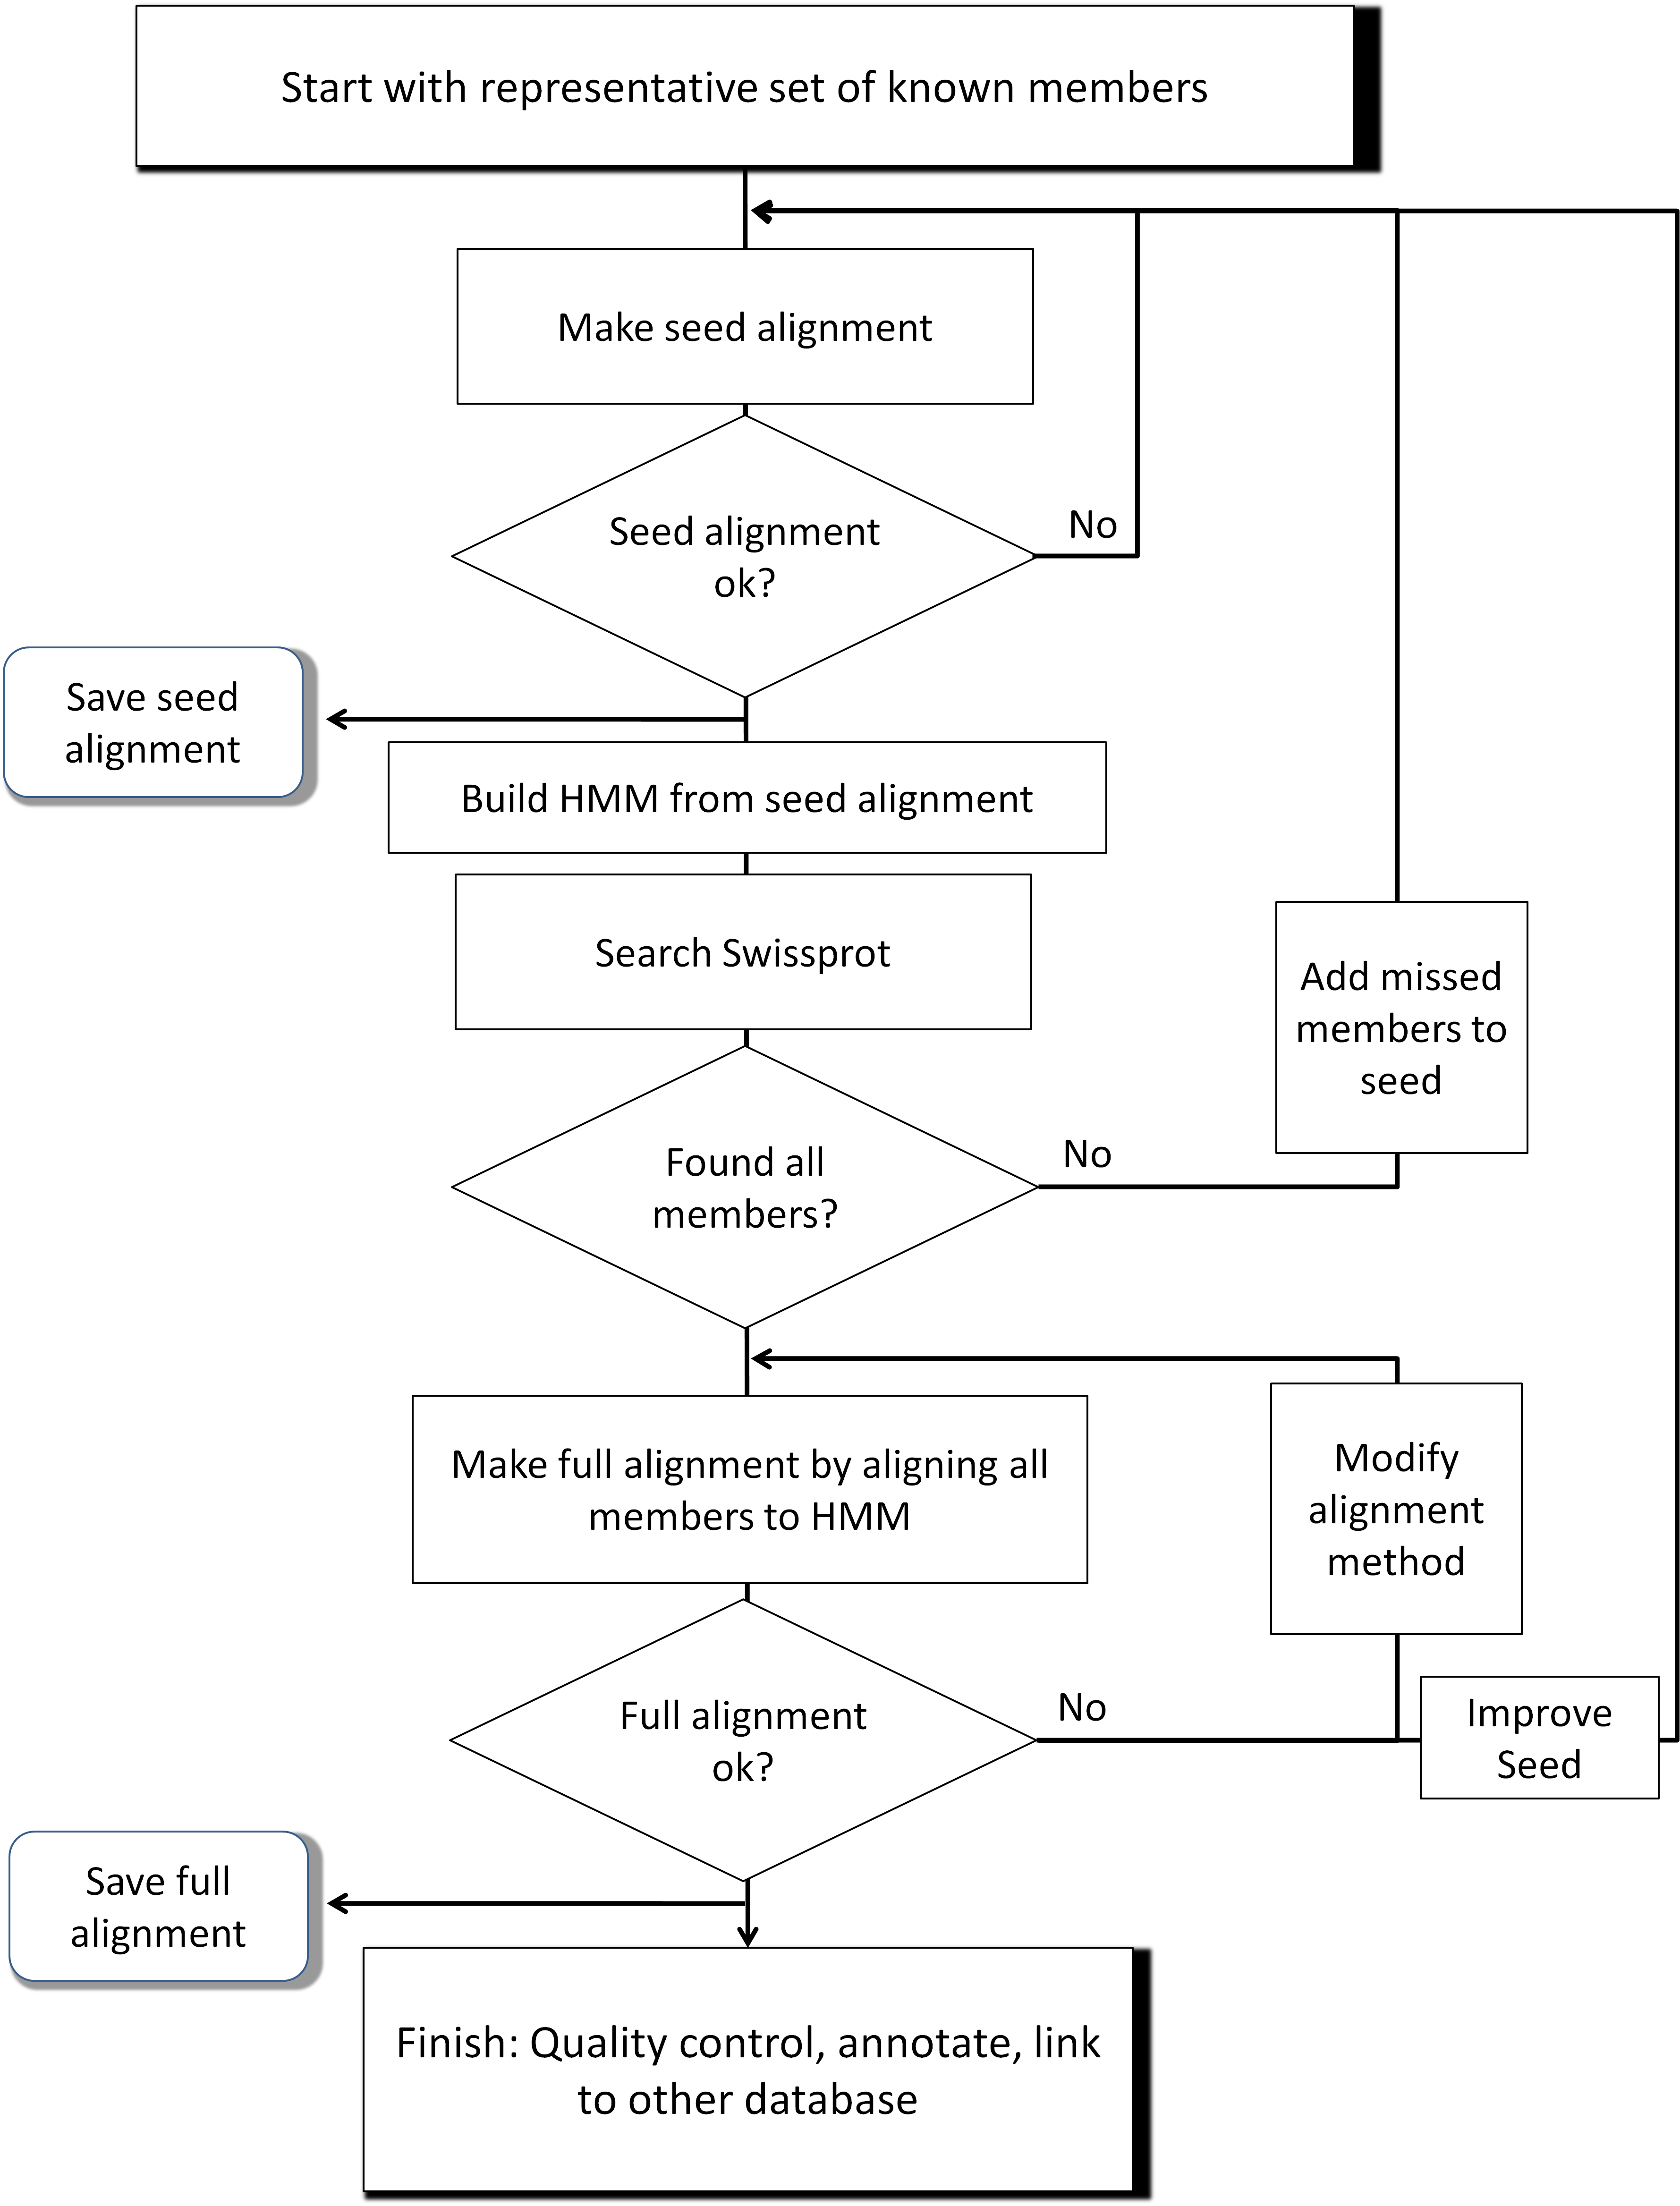
\includegraphics[width=.95\textwidth]{Pfam_workflow.png}
\caption{Abgebildet ist der \ac{Pfam} Daten Workflow, welcher die Schritte von einem repräsentativen Set bekannter Mitglieder, über das \emph{SEED} bis zum vollständigen Alignment zeigt, aus \cite{Mathias.2014}.}
\label{fig:Pfam_workflow}
\end{figure}

Die Pfam wurde 1997 von Sonnhammer EL, Eddy SR und Durbin R. ins Leben gerufen \cite{Sonnhammer.1997}. Ihr Ziel war es eine Datenbank zur Proteinsequenzklassifizierung und -analyse zu erschaffen. Die Pfam setzt sich aus zwei Teilen zusammen, der Pfam A und Pfam B. Die Pfam-A ist kuratiert und enthält gut charakterisierte Protein Domain Familien mit hochqualitativen Alignments. Dies wird durch manuell überprüften Seed Alignments und HMMs gewährleistet. Pfam B hingegen enthält Sequenzfamilien, bei denen der Domainer Algorithmus zum Alignieren und Clustern, aller nicht Pfam A Sequenzen, genutzt wurde. 

Die aktuelle Version ist Pfam 31.0 und wurde am Europäischen Bioinformatik Institut (EBI)\footnote{\url{https://www.ebi.ac.uk}} produziert, mittels einer Sequenzdatenbank namens Pfamseq, welche auf UniProt\footnote{\url{http://www.uniprot.org}} basiert. Sie enthält aktuell 16712 Familien in 607 Clans (März 2017).


\newpage
\subsection{ClinVar}
\label{sec:clinvar}
Die ClinVar\footnote{\url{https://www.ncbi.nlm.nih.gov/clinvar/}} Datenbank enthält Informationen über genetische Variationen und deren Auswirkungen auf die menschliche Gesundheit. Die Variationen sind in verschiedene Kategorien aufgeteilt, wie in Kapitel \ref{sec:snp_exp} beschrieben. Zum Zeitpunkt dieser Arbeit (Oktober 2017) enthielt sie 82.147 als \emph{pathogenic} markierte und 105.337 als \emph{benign} markierte genetische Variationen. Diese Daten wurden von 838 Autoren\footnote{\url{https://www.ncbi.nlm.nih.gov/clinvar/docs/submitter_list/}} eingetragen, die Top 10 sind in Tabelle \ref{tab:clinvar} eingetragen.

\begin{table}[H]
    \centering
    \caption{Dargestellt sind die Top 10 Autoren der ClinVar sortiert nach der Anzahl ihrer Beiträge in die Datenbank.}
    \label{tab:clinvar}
    \resizebox{\linewidth}{!}{%
    \begin{tabular}{llll}
        \hline
        \multicolumn{1}{|l|}{Autor} & \multicolumn{1}{l|}{Beiträge} & \multicolumn{1}{l|}{Interpretationen} & \multicolumn{1}{l|}{Gene} \\ \hline
        Illumina Clinical Services Laboratory; Illumina & 138336 & 138336 & 2085 \\
        GeneDx & 73416 & 73098 & 22930 \\
        Invitae & 45422 & 41425 & 698 \\
        EGL Genetic Diagnostics; Eurofins Clinical Diagnostics & 30127 & 30097 & 1772 \\
        OMIM; Johns Hopkins University & 28264 & 28264 & 4379 \\
        Ambry Genetics & 21422 & 21422 & 435 \\
        Laboratory for Molecular Medicine; HealthCare Personalized Medicine & 19020 & 18930 & 1351 \\
        PreventionGenetics & 15739 & 15739 & 1491 \\
        Genetic Services Laboratory; University of Chicago & 15340 & 15340 & 1212 \\
        Database of Curated Mutations; Washington University in St Louis & 6947 & 6878 & 131
        \end{tabular}}
\end{table}

Um die Qualität der Annotation zu bewerten, gibt es den sogenannten \emph{Review Status}, dieser gibt an wie gut die Annotation ist. So gibt es z.B. einen Stern, wenn die genetische Variation bisher nur von einem Autor eingetragen wurde. Gibt es mehrere Autoren und widersprechen sich die Annotationen nicht, so bekommt die Annotation zwei Sterne. Die fast beste Qualität, mit drei Sternen, hat das \emph{expert panel}, Autoren in dieser Kategorie müssen spezielle Anforderungen erfüllen\footnote{\url{https://www.ncbi.nlm.nih.gov/clinvar/docs/review_guidelines/}}. Die beste Annotation mit vier Sternen hat \emph{practice guideline}. Für diese Arbeit wurde auf alle Daten, von zwei bis vier Sternen, zugegriffen.



\section{Bewertungen von Klassifikationen}
In dieser Arbeit war es wichtig, die vorhergesagten Klassifikationen zu bewerten. Dabei hängt die Güte des Klassifikators von dessen Typ ab. In diesem Fall handelt es sich um einen binären Klassifikator, daher können zwei Bewertungsverfahren in Betracht gezogen werden.

\subsection{F1 Score}
Der F1 Score ist ein statistisches Maß, um die Testgenauigkeit zu bewerten. Er verwendet sowohl die \emph{Präzision} p, als auch den \emph{Recall} r, um den Score zu berechnen. P ist die Anzahl aller richtigen positiven Ergebnisse, geteilt durch die Anzahl an allen positiven Ergebnissen. R ist die Anzahl an vorhergesagten richtigen positiven Ergebnissen, geteilt durch die Anzahl der tatsächlich positiven Ergebnisse, vgl. Formel \ref{eq:f1_score}.
\begin{equation}
    F_{1} = 2 \times \frac{1}{\frac{1}{recall}+\frac{1}{precision}} = \frac{\text{precision} \times \text{recall}}{\text{Precision} + \text{recall}}
    \label{eq:f1_score}
\end{equation}

Der F1 Score kann Werte von 0 bis 1 annehmen, wobei ein Score von 1 die beste mögliche Aussage bedeutet.


\subsection{Matthews correlation coefficient}
\label{sec:mcc}
Der \emph{Matthews correlation coefficient}, oder kurz MCC ist ein Maß um die Qualität einer binären Klassifikation zu bewerten und wird oftmals im Bereich des \emph{Machine Learnings} angewandt. Der Biochemiker Brian W. Matthews führte diesen Algorithmus 1975, in seinem Paper „Comparison of the predicted and observed secondary structure of T4 phage lysozyme“ \cite{Matthews.1975} ein. Der MCC berücksichtig \emph{true} und \emph{false postives}, sowie \emph{true} und \emph{false negatives}, um eine Bewertung einer beobachteten und vorhergesagten zwei Klassen Klassifizierung zu treffen. Dabei kann der MCC einen Wert von -1 bis 1 annehmen. Ein Koeffizient von 1 repräsentiert eine perfekte Vorhersage. Ein Koeffizient von 0 bedeutet, dass die Vorhersage nicht besser ist, als ein zufälliger Münzwurf. Ein Wert von -1 deutet auf eine totale Differenz zwischen Beobachtung und Vorhersage hin. Der MCC ist auch bekannt als Phi Koeffizient und zusammenhängend mit der chi Quadrat Statistik, für eine 2x2 Kontingenztabelle, in der n für die totale Anzahl der Beobachtungen steht.

\begin{equation}
    |MCC| = \sqrt{\frac{x^2}{n}}
    \label{eq:mcc}
\end{equation}

Der MCC gilt als ausbalanciertes Maß, selbst wenn die Klassen sehr verschiedene Größen haben, andere Maße, wie der einfache „Anteil der richtigen Vorhersagen“, auch bekannt als statistische Genauigkeit, sind nicht sehr aussagekräftig, wenn zwei Klassen unterschiedlich groß sind. Denn wenn jedes Objekt dem größeren Set zugewiesen wird, so erreicht man eine höhere Anzahl an korrekten Vorhersagen, welche statistisch gesehen allerdings wenig Aussagekraft besitzen.

Der MCC berechnet sich direkt aus der Konfusionsmatrix Tabelle \ref{table:konfusionsmatrix}, mit der Formel \ref{eq:mcc2}:

\begin{table}[H]
    \centering
    \caption{Dargestellt ist die Konfusionsmatrix. tp = \emph{true positives}, fp = \emph{false postives}, tn \emph{true negatives} und fn = \emph{false negatives}.}
    \label{table:konfusionsmatrix}
    \resizebox{\linewidth}{!}{%
    \begin{tabular}{l|l|l|}
        \cline{2-3}
         & pathogenic SNP (tp + fn) & benign SNP (fp + tn) \\ \hline
        \multicolumn{1}{|l|}{test positive (tp + fp)} & \cellcolor[HTML]{9AFF99}true positive (tp) & \cellcolor[HTML]{FFCCC9}fals positive (fp) \\ \hline
        \multicolumn{1}{|l|}{test negative (fn + tn} & \cellcolor[HTML]{FFFFC7}false negative (fn) & \cellcolor[HTML]{9AFF99}true negative (tn) \\ \hline
    \end{tabular}}
\end{table}

\begin{equation}
    MCC = \frac{TP \times TN - FP \times FN}{\sqrt{(TP + FP)(TP + FN)(TN + FP)(TN + FN)}}
    \label{eq:mcc2}
\end{equation}

In Gleichung \ref{eq:mcc2} ist TP die Anzahl der \emph{true postives}, TN die Anzahl der \emph{true negatives}, FP die Anzahl der \emph{true postives} und FN die Anzahl der \emph{true negatives}. Wenn eine der 4 Summen im Teiler 0 ergibt, so kann man den Nenner willkürlich auf 1 setzen, sodass man einen MCC von 0 erhält, dies stellt den Grenzwert der Gleichung dar.


\section{Homologie Berechnung}
\label{sec:siwssmodel}
Im Rahmen dieser Arbeit war es nötig 3D-Strukturen für Proteinsequenzen zu ermitteln, welche nicht oder nur teilweise aufgeklärt sind. Homologieberechunungen werden häufig eingesetzt, wenn es keine experimentellen Daten zu einer Struktur eines Proteins gibt.
\begin{figure}[H]
    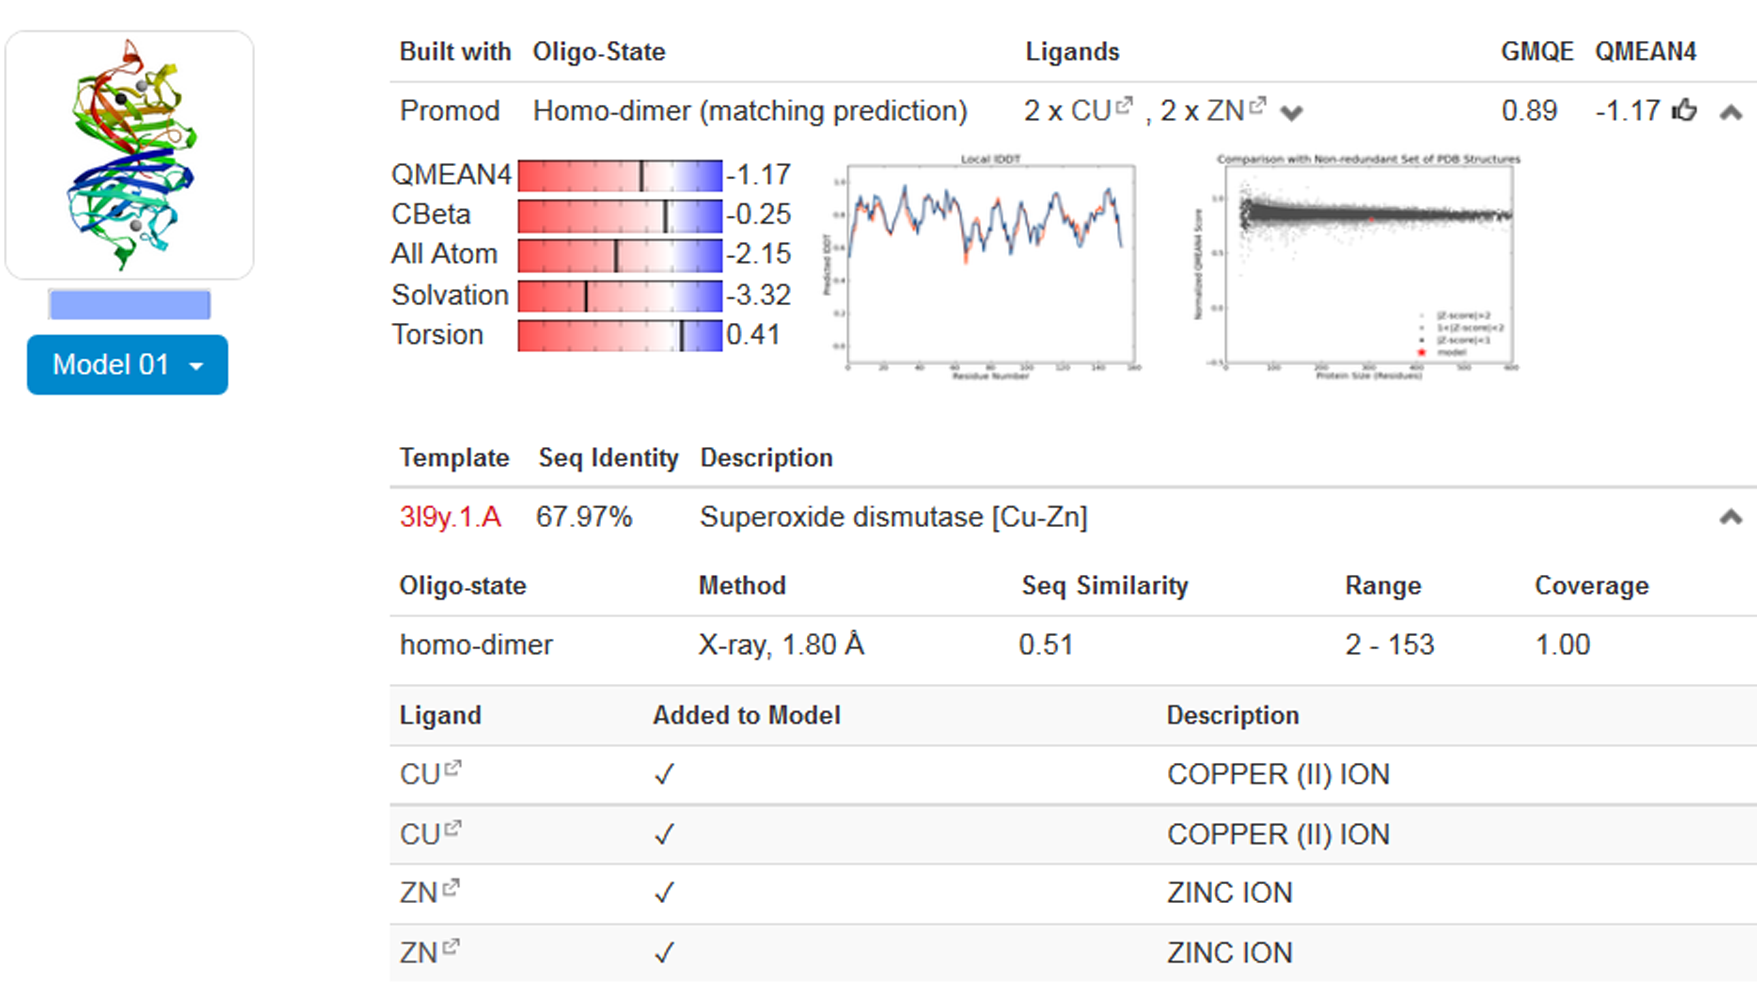
\includegraphics[width=.95\textwidth]{images/Swissmodel.png}
    \caption{Beispielhaftes Ergebnis einer Swissmodelanfrage, für jedes Modell werden Koordinaten, Alignment, Sequenzidentität, Abdeckung, Modellierungsprotokoll, eine Qualitätsschätzung und vieles mehr zur Verfügung gestellt.}
    \label{fig:swissmodel}
\end{figure}

\begin{quote}
    "Die Homologiemodellierung (oder vergleichende Modellierung) stützt sich auf evolutionär verwandte Strukturen (Templates) zur Generierung eines Strukturmodell eines Proteins von Interesse (Target). Der Prozess umfasst typischerweise die folgenden Schritte: (i) Vorlage Identifikation, (ii) Auswahl der Vorlagen, (iii) Modellerstellung und (iv) Schätzung der Modellqualität. Kurz gesagt, eine Bibliothek von experimentell ermittelten Proteinstrukturen wird gesucht, mit empfindlichen Sequenzsuchwerkzeugen zur Identifizierung von Proteinen, die evolutionär mit dem Zielprotein verwandt sind. Wenn eine oder mehrere Vorlagen identifiziert sind, werden die Informationen der Abgleich der Ziel- und Modell-Sequenzen gemeinsam mit den 3D-Koordinaten der Vorlage (n) verwendet, um ein Strukturmodell für das Protein zu erstellen. Schließlich wird die Qualität des berechneten Modells geschätzt, um die Qualität des berechneten Modells für spätere Anwendungen zu zeigen."
\end{quote}

Übersetzt aus \cite{Biasini.2014}, den Autoren des Webservers Swissmodel\footnotetext{\url{https://swissmodel.expasy.org}}, welcher zur Homologie Berechnung genutzt wurde. Swissmodel liefert nach der Berechnung eine 3D-Struktur, mit einer gewissen \emph{Coverage}. Die Coverage bezeichnet den prozentualen Anteil der Struktur, welcher für die gegebene Aminosäuresequenz berechnet wurde. Je höher die Coverage ist, desto vollständiger ist also die Proteinstruktur.

Swissmodel zeichnet sich durch eine aufgeräumte Benutzeroberfläche, einem zuverlässig Server und einer schnellen Berechnung aus, siehe \ac{Abb} \ref{fig:swissmodel}. Zudem ist kein Download erforderlich und dadurch wurde auch keine Referenzdatenbanken benötigt. Damit war der Webserver die optimale Wahl für diese Arbeit.



\section{Ramachandran Plot}
\label{sec:ramachandran}
Der Ramachandran Plot wurde 1963 von G. N. Ramachandran \cite{RAMACHANDRAN.1963} entwickelt, um die jeweiligen Diederwinkel (oder auch Torsionswinkel)  $\psi\ \&\ \phi$ eines bestimmten Protein-Backbones darzustellen. Die 3D-Struktur eines Proteins wird hauptsächlich durch nicht kovalente Bindungen zwischen Atomen unterschiedlicher Aminosäurereste bestimmt. Diese Bindungen sind für Strukturen wie Alpha Helices und Beta Faltblätter verantwortlich. Dies wird durch Veränderungen der  $\psi\ \&\ \phi$ Winkel des C Alpha Atoms erreicht, denn durch den Doppelbindungscharakter der Aminosäuren ist der $\omega$ Winkel immer 180° und das Protein damit planar. Somit können sich $\psi\ \&\ \phi$ Winkel in einem Bereich von -180° bis +180° befinden, siehe \ac{Abb} \ref{fig:psi_phi}. Wenn man nun auf der Ordinate die $\psi$-, auf der Abszisse die $\phi$-Winkel der C Alpha Atome aufträgt, erhält man den typischen Ramachandran Plot. 

\begin{figure}
    \centering
    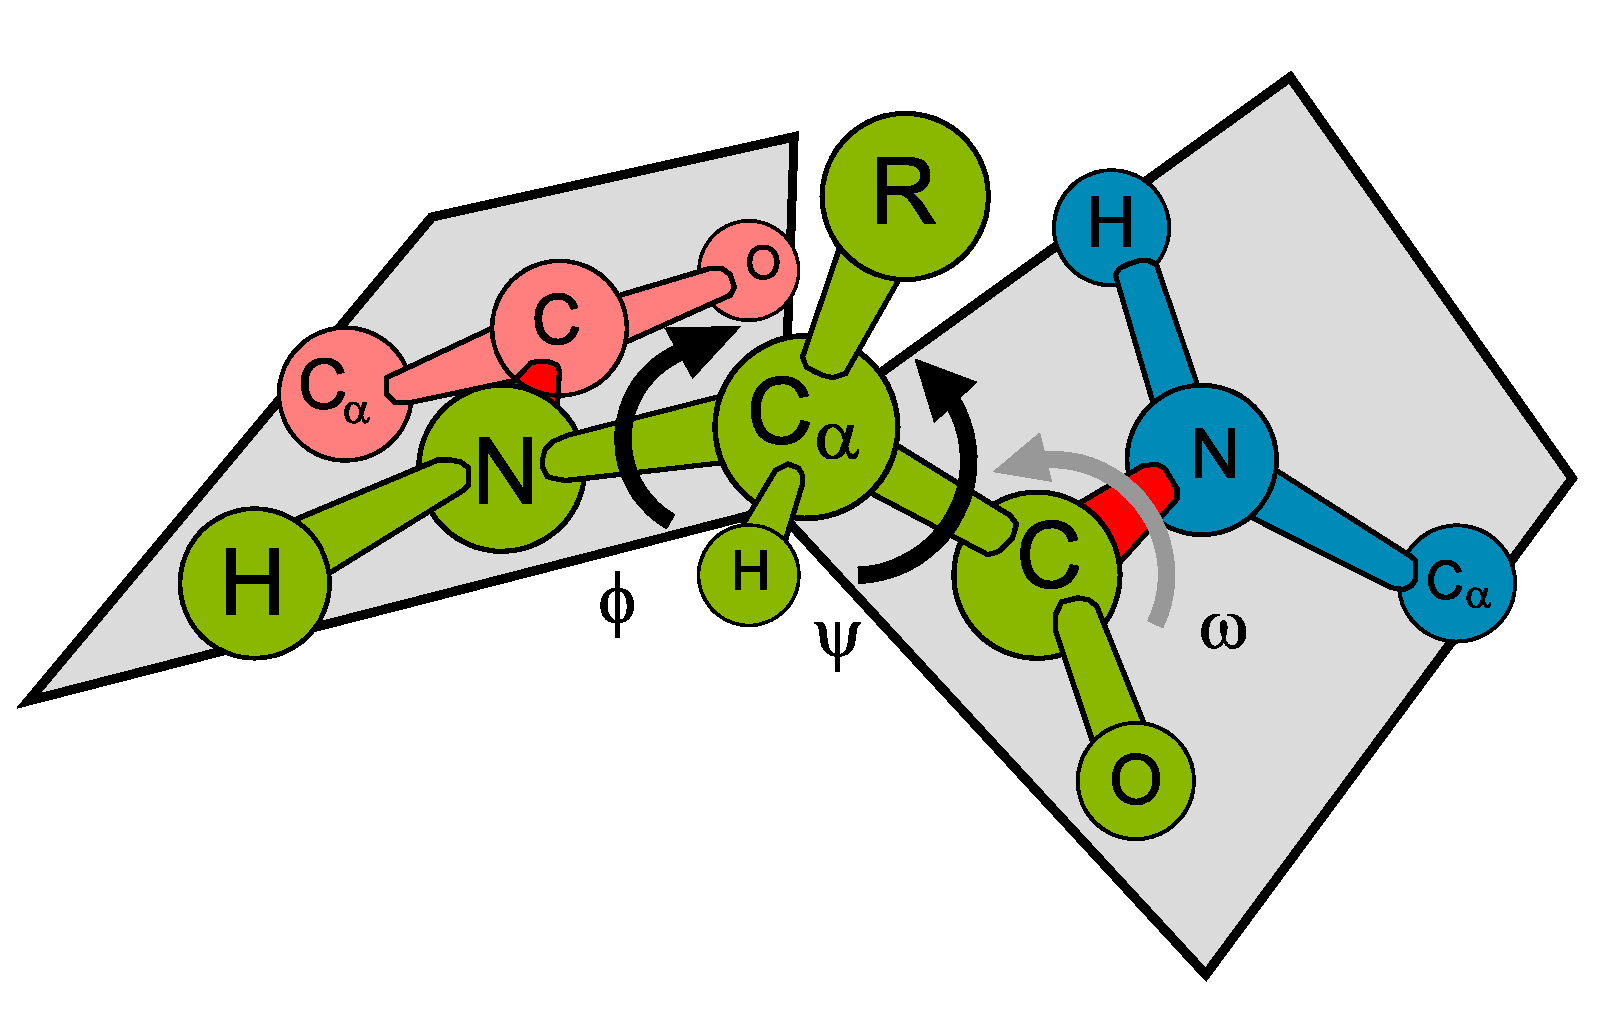
\includegraphics[width=.95\textwidth]{psi_phi.png}
    \caption{2-dimensionale Projektion eines Proteins mit C $\alpha$ Atom in der Mitte und gekennzeichneten Winkeln. Die grauen Ebenen zeigen, dass die Atome, welche durch die Peptidbindung (rot) verbunden sind, jeweils auf einer Ebene liegen, so kann sich der Aminosäurerest (grün) über seine $\psi\ \&\ \phi$ Winkeln frei drehen. Die Amino-Gruppe ist blau und die Carboxyl-Gruppe ist rosa dargestellt.\protect\footnotemark}
    \label{fig:psi_phi}
\end{figure}
\footnotetext{\url{https://application.wiley-vch.de/HOME/bioinformatik/prot/Prot_1d/ueb/pepbind.png}}

Anhäufungen im Ramachandran Plot sind immer charakteristisch für spezifische Protein-Sekundärstrukturen, wie z.B. alpha Helices oder beta Faltblätter. Diese sind in der Abbildung \ref{fig:ramaplot} zu sehen.

\begin{figure}[H]
    \centering
    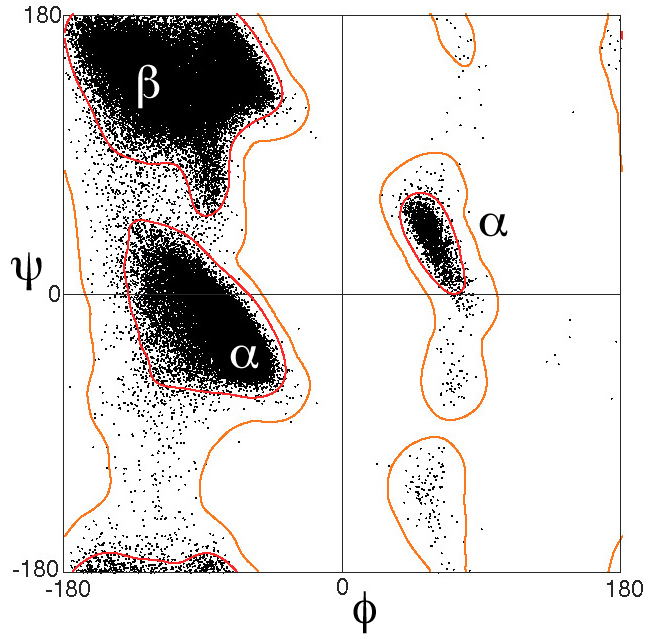
\includegraphics[width=.80\textwidth]{images/Ramaplot.png}
    \caption{Abgebildet ist ein Ramachandran Plot welcher 100.000 representative Datenpunkte darstellt. Gut zu sehen sind die Akkumulationen, der rechts ($\alpha$) und links ($\alpha'$) drehenden alpha-Helices, sowie die beta-Faltblätter ($\beta$). Auf der Ordinate sind die PSI-, auf der Abszisse die PHI-Winkel aufgetragen\protect\footnotemark.}
    \label{fig:ramaplot}
\end{figure}
\footnotetext{\url{http://proteopedia.org/wiki/index.php/Ramachandran_Plots}}

Mathematisch lässt sich der Ramachandran Plot mit folgender Gleichung beschreiben:

\begin{equation}
    f : [-\pi,\pi]\times[-\pi,\pi] \rightarrow \R_{+}
    \label{eq:rama_eq}
\end{equation}



\section{Durchführung der Berechnungen}


\subsection{Apache Spark}
In dieser Arbeit wurde mit der gesamten RCSB \ac{PDB} und somit mit 133.277 Energieprofilen gearbeitet. Um diese Datenmasse adäquat und schnell zu verarbeiten, wurde sowohl eine Hardware, als auch Software Lösung benötigt, da ein normaler PC nicht mehr ausreicht, diese Datenmengen zeitnah zu verarbeiten. Hierzu wurde als Hardwarelösung das Cluster der Arbeitsgruppe Goesmann genutzt, indem auf 5000 virtuelle Kerne mit 512GB RAM zugegriffen wurde. 

\begin{figure}[H]
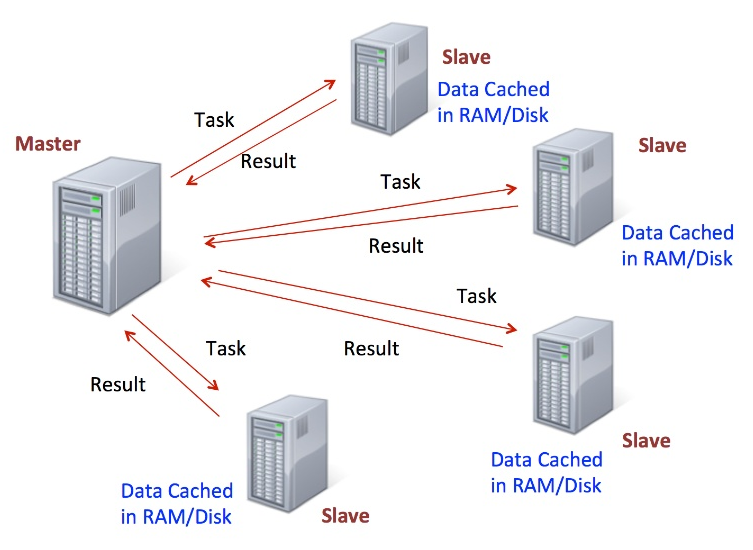
\includegraphics[width=.95\textwidth]{apache_spark.png}
\caption{Dargestellt ist die Apache Spark Job Ausführung, zwischen Master und Slave Computern im Netzwerk. Der Master verteilt Aufgaben an die Slave Rechner, welche wiederum die Ergebnisse zurück an den Master Computer senden, \ac{Abb} geändert nach\protect\footnotemark.}
\label{fig:apache_spark}
\end{figure}
\footnotetext{\url{https://www.slideshare.net/perone/apache-spark-intro-to-largescale-recommendations-with-apache-spark-and-python}}

Als Softwarelösung wurde Apache Spark\footnote{\url{https://spark.apache.org}} eingesetzt. Hierbei handelt es sich um eine general-purpose Cluster Software, welche über eine High Level API in Python, Scala, R und Java verfügt. Gerade die Python API war sehr hilfreich, da die Mehrzahl aller Skripte für diese Arbeit in Python geschrieben wurden. So konnte ein Python Skript erst lokal auf einem PC entwickelt und mit einem Testdatensatz überprüft werden, um es anschließend mit Spark auf dem Cluster der AG Goesmann zu deployen. Nach dem Deployment verteilt Spark die Daten automatisch auf dem Cluster und fängt die Ergebnisse ab, siehe \ac{Abb} \ref{fig:apache_spark}. 

Zudem verfügt Spark noch über ein SQL Tool zum Verarbeiten von strukturierten Daten, MLib für Machine Learning und GraphX für Graph Prozessierung.



\newpage
\subsection{Nextflow}

\begin{wrapfigure}{R}{0.5\textwidth}
    \centering
    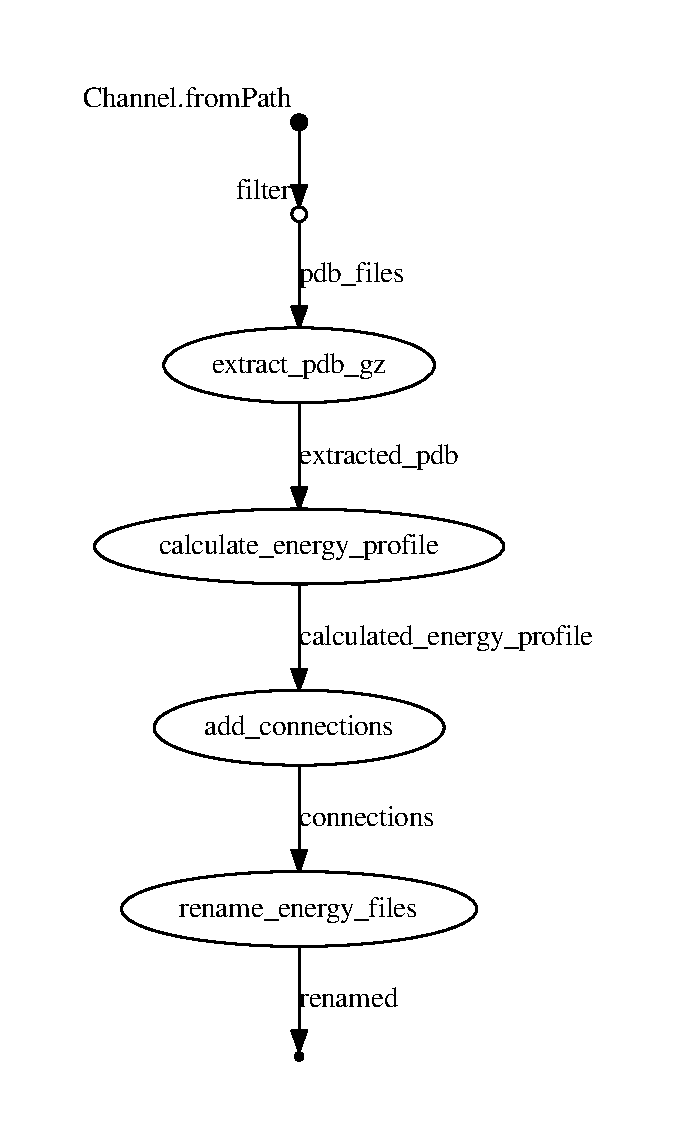
\includegraphics[width=0.45\textwidth]{images/flowchart.pdf}
    \caption{Ablauf der Nextflow Pipeline dieser Arbeit, jedes Oval stellt einen Software Container dar, die Channel Namen sind an den Pfeilen zu sehen.}
    \label{fig:nextflow_pipe}
\end{wrapfigure}
Bei Nextflow\footnote{\url{https://www.nextflow.io}} handelt es sich um \emph{data-driven computational} Pipelines, mit denen man leicht Workflows parallelisieren kann. Mit Nextflow lassen sich leicht skalierbare und reproduzierbare wissenschaftliche Workflows schreiben, indem man mit Software Containern arbeitet. Der wesentliche Vorteil dieser Container ist, dass man sie in jeder beliebigen Programmiersprache schreiben kann. So wird in dieser Arbeit Nextflow verwendet, um Container mit Python und Java zu vereinen. Jeder Container hat einen Eingangs- und einen Ausgangs- \emph{Channel}, also einen Fluss an Daten. Zudem kann eine Pipeline wie in \ac{Abb} \ref{fig:nextflow_pipe} dargestellt, linear ablaufen oder sich verzweigen.

Eine weitere Stärke von Nextflow ist, das man alle Pipelines nicht nur auf dem lokalen Computer ausführen kann, sondern z.B. mit \texttt{drmaa} auf einem Cluster oder in der Cloud. So lassen sich auch große Datensätze und rechenintensive Aufgaben zeitnah bewältigen.


%\textbf{Auf der Webseite stehen noch Buzzwords wie: \emph{Fast prototyping, Portable, Continuous checkpoints, Unified parallelism, Stream oriented}}



\section{Python}
Der Hauptteil der benötigten Programme dieser Arbeit wurde in Python\footnote{\url{https://www.python.org}} geschrieben. Python zeichnet sich durch eine klare und Objekt orientierte Syntax aus. Es ist vergleichbar mit Perl, Ruby, Scheme oder Java. Python ist gut dokumentiert und gehört zu den Programmiersprachen die weithin als leicht zu erlernen gelten, dies macht es ideal für ad-hoc Programmieraufgaben und Prototyping, wie es in dieser Arbeit gefordert wurde. Außerdem läuft Python auf allen Betriebssystemen wie Mac OS X, Windows und Unix. Python ist zusätzlich komplett \emph{Open Source} und damit akademisch komplett entgeltfrei nutzbar.

Durch meine Entwicklertätigkeit im EDGAR \cite{Yu.2017} Projekt der JLU hatte ich viel Kontakt mit Perl und der Unix Umgebung, damit war Python die logische Wahl der Programmiersprache für diese Arbeit.

Es wurde die Python \emph{legacy} Version 2.7 verwendet. Diese zeichnet sich dadurch aus, dass es zu diesem Zeitpunkt noch mehr Bibliotheken für diese Version gibt als für Python 3.X, was der fehlenden Abwärtskompatibilität geschuldet ist. So wurde in dieser Arbeit z.B. mit den Bibliotheken \texttt{Matplotlib}\footnote{\url{https://matplotlib.org}} und \texttt{Seaborn}\footnote{\url{http://seaborn.pydata.org}} gearbeitet um Daten zu visualisieren.

In Python 3 wurde die Programmiersprache grundlegend überarbeitet. Das hat im Wesentlichen zu einem viel besseren Unicode Support, sowie einer standardmäßigen \emph{bytes/Unicode} Separierung geführt. Zudem wurde die gesamte Konsistenz der Programmiersprache verbessert, das war aber nicht relevant für diese Arbeit.
